\chapter{Von Ising-Magneten zur kritischen Zustandsänderung zwischen Flüssigkeit und--Gas}

\lectureoverview{Der Übergang zwischen Flüssigkeit und--Gas lässt sich auf einem unerwarteten Weg erreichen. Zunächst vervollständigen wir die Mean-Field-Behandlung des Ising-Magneten und bestimmen seine Koexistenzlinie und seinen kritischen Punkt. Anschließend deuten wir einen Spin nach oben als besetzten Gitterplatz. Das so entstehende Gittergas weist einen harten Kern, kurzreichweitige Anziehung und ein vom Magnetfeld gesteuertes chemisches Potenzial auf und besitzt genau dasselbe Phasendiagramm. Der formale Teil der Vorlesung schließt mit kritischem Verhalten und Universalität. In einer gesonderten Diskussion im Anschluss an die Vorlesung geht es darum, was Physiker unter Feinabstimmung verstehen, wie Selektionseffekte in Erklärungen eingehen können und warum solche Überlegungen nur dann nützlich sind, wenn sie mit einem Mechanismus und möglichen Tests verknüpft werden.}

\section{Warum das Verständnis siedenden Wassers mit einem Magneten beginnt}

Siedendes Wasser ist das vertraute Phänomen, das wir verstehen möchten: Eine Flüssigkeit geht in ein Gas über, und ihre Dichte ändert sich sprunghaft. Der übliche Zugang führt über die van-der-Waals-Gleichung. Hier wählen wir einen anderen Weg. Wir kehren zum Ising-Magneten zurück, vervollständigen seine Mean-Field-Beschreibung und erkennen dann, dass sich dasselbe Modell auch als Fluid deuten lässt.

Das ist mehr als eine anschauliche Analogie. Sind die Variablen richtig übersetzt, beschreiben der Ising-Magnet und das Gittergas dasselbe statistisch-mechanische System. Die Magnetisierung wird zur Teilchendichte, das äußere Magnetfeld zum chemischen Potenzial und die magnetische Koexistenzlinie zur Koexistenzlinie zwischen Flüssigkeit--Gas. Diese Übersetzung erklärt, warum zwei scheinbar unterschiedliche Materiesysteme dasselbe kritische Verhalten zeigen können.

In niedrigen Dimensionen liefert die Mean-Field-Näherung keine exakten Zahlenwerte. In einer Dimension sagt sie sogar einen Übergang voraus, den die exakte Lösung ausschließt. Ihr Wert liegt hier in der Struktur. In zwei und drei Dimensionen zeigt sie den richtigen Ordnungsparameter, die konkurrierenden Phasen, den kritischen Endpunkt und wie eine infinitesimale Bevorzugung eine Phase auswählt. In drei Dimensionen, wo jeder Gitterplatz sechs nächste Nachbarn hat, ergibt sich bereits ein nützliches qualitatives Bild, wenn man diese Nachbarn durch ihren Mittelwert ersetzt.

\section{Die Energiebilanz des Ising-Modells}

Wir setzen auf jeden Platz eines hyperkubischen Gitters einen Spin mit zwei möglichen Zuständen,
\begin{equation}
\sigma_i=\pm1.
\end{equation}
und verwenden den Hamiltonoperator
\begin{equation}
\mathcal H
=-J\sum_{\langle ij\rangle}\sigma_i\sigma_j
+h\sum_i\sigma_i,
\qquad J>0.
\label{eq:ising-hamiltonian}
\end{equation}
Die Notation ist wichtig. Die erste Summe läuft über nächste-Nachbar-\emph{Bindungen}, die zweite über \emph{Gitterplätze}. Jede Bindung wird einmal gezählt, nicht je einmal von ihren beiden Endpunkten aus.

Für eine einzelne Bindung gilt
\begin{equation}
E_{ij}=-J\sigma_i\sigma_j.
\end{equation}
Parallele Spins haben die Energie \(-J\), antiparallele Spins die Energie \(+J\). Eine gebrochene Bindung kostet daher
\begin{equation}
\Delta E_{\rm bond}=+J-(-J)=2J.
\label{eq:broken-bond}
\end{equation}
Die Größe \(2J\) und nicht eine der absoluten Bindungsenergien bestimmt die relativen Boltzmann-Gewichte. Wir könnten zu jeder Konfiguration dieselbe Konstante addieren, ohne eine Wahrscheinlichkeit zu ändern.

\begin{classroomqa}
\audiencequestion{Warum gibt es im Hamiltonoperator zwei verschiedene Summen?}
\lecturerresponse{Die Austauschenergie gehört zu einem Paar benachbarter Gitterplätze und wird daher über Bindungen summiert \(\langle ij\rangle\). Das Feld wirkt unabhängig auf jeden Spin und wird deshalb über Gitterplätze summiert \(i\). Werden diese beiden Zählweisen verwechselt, entstehen genau die Faktoren 2, die in der Mean-Field-Näherung eine Rolle spielen werden. \lecturetimestamp{00:08:04--00:08:45}}
\end{classroomqa}

\begin{classroomqa}
\audiencequestion{Bedeutet ein größeres \(J\) einfach, dass jede Energie negativer wird?}
\lecturerresponse{Es vergrößert den Energieunterschied zwischen parallelen und nicht parallelen Konfigurationen. Der Nullpunkt der Energie ist beliebig; die physikalische Aussage ist, dass eine gebrochene Bindung \(2J\) kostet. Ein größeres positives \(J\) macht thermische Unordnung daher bei fester Temperatur weniger günstig. \lecturetimestamp{00:08:47--00:10:17}}
\end{classroomqa}

Auf einem unendlichen oder periodischen hyperkubischen Gitter in \(d\) Dimensionen hat jeder Gitterplatz \(2d\) Nachbarn. Zählt man von allen \(N\) Gitterplätzen aus, wird jede Bindung zweimal gezählt, also
\begin{equation}
N_{\rm links}=\frac{(2d)N}{2}=dN.
\label{eq:number-links}
\end{equation}
Eine vollständig ausgerichtete Konfiguration hat folglich die Austauschenergie \(-JdN\). Randplätze bewirken eine Korrektur von der Größenordnung eines Oberflächenterms, der im thermodynamischen Limes gegenüber \(N\) vernachlässigbar ist. Bei \(h=0\) sind die beiden vollständig ausgerichteten Zustände entartet.

Der Feldterm legt eine Vorzeichenkonvention fest, die wir durchgehend beibehalten. In Gleichung~\eqref{eq:ising-hamiltonian} führt ein positives \(h\) zu einer niedrigeren Energie am Gitterplatz für \(\sigma=-1\). Daher begünstigt \(h>0\) eine negative Magnetisierung, während \(h<0\) eine positive Magnetisierung begünstigt. Man kann diese Konvention umkehren, indem man \(-h\sum_i\sigma_i\) schreibt; physikalisch ändert sich dadurch nichts, aber dann müssen alle späteren Vorzeichen ebenfalls umgekehrt werden.

\begin{classroomqa}
\audiencequestion{Wo kommt die Temperatur ins Spiel, wenn der Hamiltonoperator nur \(J\) und \(h\) enthält?}
\lecturerresponse{Die Temperatur geht über den Boltzmann-Faktor \(e^{-\beta\mathcal H}\) ein, wobei \(\beta=1/T\) in Einheiten \(k_{\rm B}=1\) gilt. Die dimensionslosen Größen sind also \(\beta J\) und \(\beta h\). \lecturetimestamp{00:13:07--00:13:43}}
\end{classroomqa}

\section{Ein Spin im mittleren Feld seiner Nachbarn}

Wir betrachten einen Spin weit entfernt vom Rand. Er hat \(2d\) nächste Nachbarn. In der Mean-Field-Näherung ersetzt man jeden fluktuierenden Nachbarspin durch denselben Mittelwert
\begin{equation}
m=\expect{\sigma}.
\end{equation}
Die Austauschenergie, an der der ausgewählte Spin \(\sigma\) beteiligt ist, lautet dann
\begin{equation}
-J\sigma\sum_{\text{\(2d\) neighbors}}\sigma_j
\;\longrightarrow\;-2dJm\,\sigma.
\end{equation}
Zusammen mit dem äußeren Feld ergibt sich die effektive Energie des einzelnen Spins:
\begin{equation}
\mathcal H_{\rm mf}(\sigma)=(-2dJm+h)\sigma.
\label{eq:mean-field-one-spin}
\end{equation}
Der Faktor \(2d\) ist entscheidend. Beim Aufstellen des Bildes mit dem zentralen Spin lässt man ihn leicht weg; bei der Herleitung an der Tafel wurde er ausdrücklich wieder ergänzt.

\begin{figure}[ht]
\centering
\includegraphics[width=0.84\textwidth]{lecture_10_figure_02.png}
\caption{Ein zentraler Spin, umgeben von seinen Mean-Field-Nachbarn, mit der Energie eines einzelnen Spins und der entstehenden Selbstkonsistenzgleichung.}
\lectureframe{00:17:57}
\end{figure}

Die Einspin-Zustandssumme lautet
\begin{align}
z_{\rm mf}
&=\sum_{\sigma=\pm1}
\exp\!\left[-\beta(-2dJm+h)\sigma\right] \\
&=2\cosh\!\left[\beta(2dJm-h)\right].
\end{align}
Der mittlere Spin ist
\begin{align}
\expect{\sigma}
&=\frac{\sum_{\sigma=\pm1}\sigma
 e^{\beta(2dJm-h)\sigma}}
{\sum_{\sigma=\pm1}e^{\beta(2dJm-h)\sigma}} \\
&=\tanh\!\left[\beta(2dJm-h)\right].
\end{align}
Der ausgewählte Spin soll jedoch typisch für die Nachbarn sein, deren Mittelwert wir mit \(m\) bezeichnet haben. Selbstkonsistenz verlangt daher
\begin{equation}
\boxed{m=\tanh\!\left[\beta(2dJm-h)\right].}
\label{eq:mean-field-self-consistency}
\end{equation}
Diese eine nichtlineare Gleichung ist die Mean-Field-Reduktion des Vielspinproblems.

\begin{classroomqa}
\audiencequestion{Warum ist der Mittelwert auf der linken Seite derselbe \(m\), den wir für jeden Nachbarn eingesetzt haben?}
\lecturerresponse{Das ist die Näherung. Wir nehmen einen homogenen Volumenzustand an, ersetzen die tatsächliche Umgebung durch ihren Mittelwert, berechnen den zentralen Spin in dieser Umgebung und verlangen, dass der berechnete Mittelwert die angenommene Umgebung reproduziert. Eine Lösung beschreibt einen selbstkonsistenten Volumenzustand. \lecturetimestamp{00:16:28--00:18:00}}
\end{classroomqa}

Wir führen ein
\begin{equation}
y=2\beta dJm.
\label{eq:y-definition}
\end{equation}
Da \(\beta=1/T\) gilt,
\begin{equation}
m=\frac{yT}{2dJ},
\end{equation}
wird Gleichung~\eqref{eq:mean-field-self-consistency} zu
\begin{equation}
\boxed{\frac{yT}{2dJ}=\tanh(y-\beta h).}
\label{eq:reduced-mean-field}
\end{equation}

\begin{figure}[ht]
\centering
\includegraphics[width=0.82\textwidth]{lecture_10_figure_03.png}
\caption{Die reduzierte Selbstkonsistenzgleichung nach Einführung von \(y=2\beta dJm\), bereit zur grafischen Lösung.}
\lectureframe{00:24:42}
\end{figure}

\begin{classroomqa}
\audiencequestion{Warum tritt das Feld als \(y-\beta h\) auf, und welchen Spin begünstigt ein positives Feld?}
\lecturerresponse{Unser Hamiltonoperator enthält \(+h\sigma\). Der Exponent im Boltzmann-Faktor lautet daher \(\beta(2dJm-h)\sigma\), sodass das Argument des hyperbolischen Tangens \(y-\beta h\) ist. Ein positives \(h\) begünstigt \(\sigma=-1\). Definiert man den Hamiltonoperator stattdessen mit \(-h\sigma\), ändert sich bei jedem Auftreten von \(h\) das Vorzeichen und das Phasendiagramm wird horizontal gespiegelt. \lecturetimestamp{00:18:17--00:20:00}}
\end{classroomqa}

\section{Grafische Lösungen und der Curie-Punkt}

Wir setzen \(h=0\). Gesucht sind die Schnittpunkte von
\begin{equation}
\frac{T}{2dJ}y
\qquad\text{and}\qquad
\tanh y.
\end{equation}
Der erste Ausdruck ist eine Gerade durch den Ursprung, der zweite eine ungerade, sättigende Kurve. Bei hoher Temperatur ist die Gerade steil und es gibt nur den Schnittpunkt \(y=0\), also \(m=0\). Mit sinkender Temperatur wird die Gerade flacher. Die kritische Temperatur ist erreicht, wenn die Gerade und der hyperbolische Tangens im Ursprung eine gemeinsame Tangente haben.

\begin{figure}[ht]
\centering
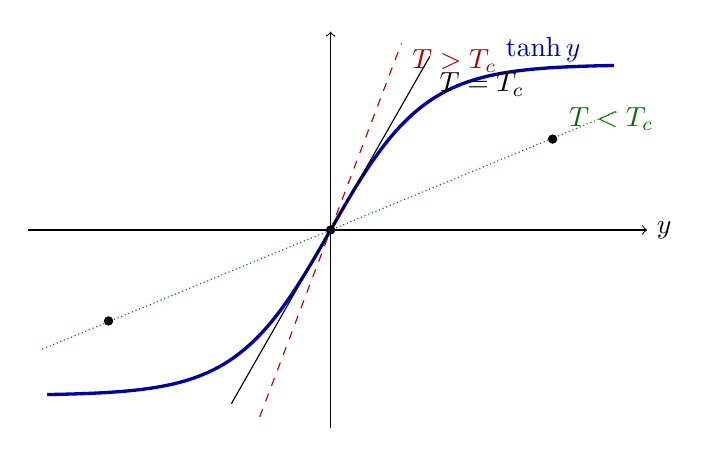
\begin{tikzpicture}[x=1.2cm,y=2.1cm]
\draw[->] (-3.2,0) -- (3.35,0) node[right] {$y$};
\draw[->] (0,-1.2) -- (0,1.2);
\draw[very thick,blue!65!black,domain=-3:3,samples=120]
  plot (\x,{tanh(\x)});
\node[blue!65!black,above] at (2.25,0.96) {$\tanh y$};
\draw[dashed,red!70!black] (-0.75,-1.13) -- (0.75,1.13);
\node[red!70!black,right] at (0.76,1.02) {$T>T_c$};
\draw[black] (-1.05,-1.05) -- (1.05,1.05);
\node[right] at (1.05,0.88) {$T=T_c$};
\draw[densely dotted,green!45!black] (-3.05,-0.72) -- (3.05,0.72);
\node[green!45!black,right] at (2.42,0.67) {$T<T_c$};
\fill (-2.35,-0.55) circle (1.7pt);
\fill (0,0) circle (1.7pt);
\fill (2.35,0.55) circle (1.7pt);
\end{tikzpicture}
\caption{Die Mean-Field-Gleichung bei verschwindendem Feld. Unterhalb von \(T_c\) entsprechen die beiden von null verschiedenen Schnittpunkte den stabilen magnetisierten Phasen; die Nulllösung bleibt algebraisch bestehen, ist aber instabil.}
\label{fig:mean-field-intersections}
\end{figure}

Da
\begin{equation}
\left.\frac{d}{dy}\tanh y\right|_{y=0}=1,
\end{equation}
lautet die Tangentialbedingung
\begin{equation}
\frac{T_c}{2dJ}=1.
\end{equation}
Somit sagt die Mean-Field-Näherung voraus:
\begin{equation}
\boxed{T_c^{\rm MF}=2dJ.}
\label{eq:sm10-mean-field-tc}
\end{equation}
Unterhalb dieser Temperatur gibt es zwei stabile, von null verschiedene Lösungen \(\pm m_0(T)\). Die Lösung \(m=0\) erfüllt die Gleichung weiterhin, entspricht aber keinem stabilen Gleichgewicht mehr. Das System wählt eine der beiden symmetrieverwandten magnetisierten Phasen.

\begin{classroomqa}
\audiencequestion{Ist das die Curie-Temperatur?}
\lecturerresponse{Ja. Bei einem Ferromagneten bezeichnet man die Temperatur, bei der die spontane Magnetisierung verschwindet, üblicherweise als Curie-Temperatur. Hier ist \(2dJ\) ihr Mean-Field-Wert, kein exaktes Ergebnis für niedrige Dimensionen. \lecturetimestamp{00:28:19--00:28:57}}
\end{classroomqa}

In der Nähe des Übergangs entwickeln wir den hyperbolischen Tangens in eine Taylorreihe:
\begin{equation}
\tanh y=y-\frac{y^3}{3}+O(y^5).
\end{equation}
Bei \(h=0\) ergibt Gleichung~\eqref{eq:reduced-mean-field}
\begin{equation}
\left(1-\frac{T}{T_c}\right)y-\frac{y^3}{3}+O(y^5)=0.
\end{equation}
Die von null verschiedenen Äste verhalten sich daher wie
\begin{equation}
y^2\simeq3\left(1-\frac{T}{T_c}\right),
\qquad
m\propto(T_c-T)^{1/2}.
\label{eq:mf-beta-exponent}
\end{equation}
Die Quadratwurzel bestimmt einen kritischen Exponenten der Mean-Field-Näherung. Sein genauer Wert bleibt in niedrigen Dimensionen nicht erhalten, aber der Ordnungsparameter verschwindet am Endpunkt weiterhin kontinuierlich.

\section{Die Temperaturfeldebene-- und Zweigauswahl}

Das Material legt \(J\) fest; die Experimentierenden können \(T\) und \(h\) variieren. Daher bietet es sich an, ein Phasendiagramm in der \(T\)--\(h\)-Ebene zu zeichnen. Unterhalb von \(T_c\) wählt ein beliebig kleines Feld einen der beiden magnetisierten Äste aus. Nach unserer Konvention wählt \(h<0\) den Zustand \(m>0\), während \(h>0\) den Zustand \(m<0\) auswählt.

Bei null Temperatur sind die Spins vollständig ausgerichtet, also gilt \(m=\pm1\). Bei hoher Temperatur ist der Mittelwert bei verschwindendem Feld \(m=0\). Nähert man sich dem kritischen Punkt entlang \(h=0\), sinkt der Betrag \(m_0(T)\) kontinuierlich auf null. Bei jedem festen \(T<T_c\) bewirkt der Übergang über \(h=0\) jedoch einen sprunghaften Wechsel von \(+m_0(T)\) zu \(-m_0(T)\).

\begin{figure}[ht]
\centering
\includegraphics[width=0.90\textwidth]{lecture_10_figure_06.png}
\caption{Die Koexistenzlinie in der \(T\)--\(h\)-Ebene und die Magnetisierungsäste bei fester Temperatur unterhalb von \(T_c\).}
\lectureframe{00:39:30}
\end{figure}

\begin{figure}[ht]
\centering
\resizebox{\linewidth}{!}{%
\begin{tikzpicture}[x=1.25cm,y=1.15cm]
\begin{scope}
\draw[->] (-2.45,0) -- (2.55,0) node[right] {$h$};
\draw[->] (0,0) -- (0,3.7) node[above] {$T$};
\draw[very thick,red!70!black] (0,0) -- (0,2.35);
\fill[red!70!black] (0,2.35) circle (2.3pt);
\node[right] at (0.08,2.35) {$T_c$};
\node at (-1.25,1.05) {$m>0$};
\node at (1.25,1.05) {$m<0$};
\draw[->,rounded corners,blue!65!black] (-1.65,0.85) -- (-1.65,3.02)
 -- (1.65,3.02) -- (1.65,0.85);
\node[blue!65!black] at (0,3.35) {continuous path};
\end{scope}
\begin{scope}[xshift=7.0cm,yshift=1.55cm]
\draw[->] (-2.5,0) -- (2.5,0) node[right] {$h$};
\draw[->] (0,-1.35) -- (0,1.4) node[above] {$m$};
\draw[very thick,blue!65!black]
  (-2.2,1.05) .. controls (-0.75,1.03) and (-0.2,0.75) .. (-0.08,0.62);
\draw[very thick,blue!65!black]
  (0.08,-0.62) .. controls (0.2,-0.75) and (0.75,-1.03) .. (2.2,-1.05);
\draw[dashed] (0,0.62) -- (0,-0.62);
\fill (0,0.62) circle (1.8pt);
\fill (0,-0.62) circle (1.8pt);
\node at (0,-1.75) {\(T<T_c\)};
\end{scope}
\end{tikzpicture}
}
\caption{Bei festem \(T<T_c\) springt die Magnetisierung beim Überqueren der Koexistenzlinie. In der vollständigen Ebene der beiden Parameter lassen sich die beiden Phasen stattdessen stetig verbinden, indem man den kritischen Punkt umgeht.}
\label{fig:ising-phase-plane}
\end{figure}

\begin{classroomqa}
\audiencequestion{Was geschieht bei genau verschwindendem Feld unterhalb von \(T_c\)?}
\lecturerresponse{Das ideale unendliche System besitzt zwei gleichwertige reine Phasen. Eine beliebig kleine verbleibende Bevorzugung, die Randbedingungen oder eine mit der Präparation verbundene Fluktuation wählen eine davon aus. Die thermodynamische Diskontinuität zeigt sich in den beiden einseitigen Grenzwerten \(m(T,0^-)=+m_0(T)\) und \(m(T,0^+)=-m_0(T)\) nach unserer Vorzeichenkonvention. \lecturetimestamp{00:35:04--00:37:10}}
\end{classroomqa}

\begin{classroomqa}
\audiencequestion{Ist das dasselbe wie Hysterese?}
\lecturerresponse{Bei Hysterese geht es um Metastabilität und die von der Vorgeschichte abhängige Verzögerung, mit der ein reales System zwischen den Ästen wechselt. Das hängt damit zusammen, erfordert aber eine über das Gleichgewichtsphasendiagramm hinausgehende Dynamik und wird hier nicht behandelt. \lecturetimestamp{00:37:11--00:37:20}}
\end{classroomqa}

\begin{classroomqa}
\audiencequestion{Können die positive und die negative Phase verbunden werden, ohne eine Diskontinuität zu überqueren?}
\lecturerresponse{Ja. Man erhöht die Temperatur über \(T_c\), ändert dort das Vorzeichen des Feldes und senkt die Temperatur anschließend wieder. Dieser Weg führt um den Endpunkt herum, und die Magnetisierung ändert sich kontinuierlich. Der Sprung ist nur dann unvermeidlich, wenn man bei festem \(T<T_c\) über \(h=0\) geht. \lecturetimestamp{00:37:20--00:38:15}}
\end{classroomqa}

\begin{classroomqa}
\audiencequestion{Nähert sich die Magnetisierung immer null, wenn \(h\) gegen null geht?}
\lecturerresponse{Nicht bei einer beliebigen Temperatur unterhalb von \(T_c\). Dort sind die einseitigen Grenzwerte von null verschieden. Die spontane Magnetisierung nähert sich nur dann null, wenn man sich der kritischen Temperatur selbst nähert. \lecturetimestamp{00:38:29--00:39:45}}
\end{classroomqa}

\section{Ein durchlässiger Behälter und das chemische Potenzial}

Nun wenden wir uns von Magneten ab und betrachten wieder Teilchen. Man stelle sich einen Bereich vor, dessen potenzielle Energie niedriger ist als die der umgebenden Räume. Die Wände sind durchlässig: Teilchen können hinein- und hinausgelangen. Ist die Energie im Inneren um den Betrag \(\mu\) niedriger, erhält die Besetzung des Inneren relativ zum Außenraum den Boltzmann-Faktor \(e^{\beta\mu}\). Wird das Potenzial dieser Mulde tiefer oder flacher, ändert sich die mittlere Teilchenzahl im Behälter.

\begin{figure}[ht]
\centering
\includegraphics[width=0.84\textwidth]{lecture_10_figure_07.png}
\caption{Das Bild eines durchlässigen Behälters in einer Potenzialmulde. Die Energiedifferenz zwischen innen und außen bestimmt, ob Teilchen den Behälter bevorzugt besetzen.}
\lectureframe{00:41:30}
\end{figure}

\begin{figure}[ht]
\centering
\resizebox{\linewidth}{!}{%
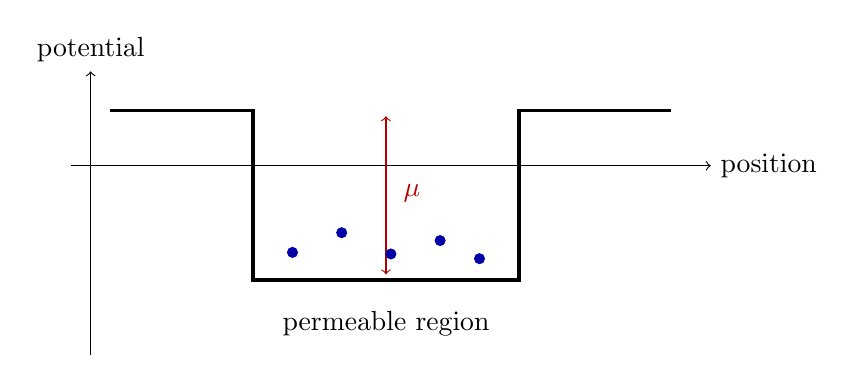
\begin{tikzpicture}[x=1.25cm,y=1.0cm]
\draw[->] (-3.2,0) -- (3.3,0) node[right] {position};
\draw[->] (-3.0,-2.4) -- (-3.0,1.2) node[above] {potential};
\draw[very thick] (-2.8,0.7) -- (-1.35,0.7)
 -- (-1.35,-1.45) -- (1.35,-1.45) -- (1.35,0.7) -- (2.9,0.7);
\draw[<->,red!70!black] (0,0.63) -- (0,-1.38);
\node[right,red!70!black] at (0.08,-0.35) {$\mu$};
\foreach \x/\y in {-0.95/-1.1,-0.45/-0.85,0.05/-1.12,0.55/-0.95,0.95/-1.18}
  \fill[blue!65!black] (\x,\y) circle (2pt);
\node at (0,-2.0) {permeable region};
\end{tikzpicture}
}
\caption{Eine Änderung des Potenzialniveaus verändert die Bevorzugung einer Teilchenzahl. In der großkanonischen Beschreibung wird dieses Niveau durch das chemische Potenzial erfasst.}
\end{figure}

Dieses Gedankenexperiment macht das chemische Potenzial anschaulich. Es ist ein Energiegewinn pro hinzugefügtem Teilchen gegenüber einem Reservoir. Können mehrere Teilchensorten die Wand passieren, hat jede Sorte ihr eigenes chemisches Potenzial. Ein abgeschlossener Behälter ist anders: Dann ist \(N\) fest, und das chemische Potenzial wird thermodynamisch bestimmt, statt durch den Austausch mit einem Reservoir vorgegeben zu sein.

\begin{classroomqa}
\audiencequestion{Ist die Tiefe der Mulde buchstäblich das chemische Potenzial?}
\lecturerresponse{Sie ist eine direkte mechanische Realisierung einer Differenz des chemischen Potenzials. Senkt man jedes Einteilchenniveau im Inneren um \(\mu\), trägt das \(-\mu N\) zur Energie und damit \(+\beta\mu N\) zum Exponenten des Boltzmann-Faktors bei. Entscheidend sind nur Differenzen des chemischen Potenzials. \lecturetimestamp{00:44:49--00:45:40}}
\end{classroomqa}

Da Teilchen ein- und austreten können, muss die Zustandssumme alle Teilchenzahlen umfassen:
\begin{equation}
\Xi(T,\mu)
=\sum_{N=0}^{\infty}\;\sum_{\mathcal C_N}
\exp\!\left[-\beta E(\mathcal C_N)+\beta\mu N\right].
\label{eq:grand-partition}
\end{equation}
Die innere Summe läuft über Konfigurationen mit festgelegtem \(N\), die äußere Summe über \(N\) selbst. Das großkanonische Gewicht lässt sich auch als \(e^{-\beta(E-\mu N)}\) schreiben.

\begin{figure}[ht]
\centering
\includegraphics[width=0.88\textwidth]{lecture_10_figure_08.png}
\caption{Der durchlässige Behälter und die großkanonische Summe über Teilchenzahlen und Konfigurationen.}
\lectureframe{00:47:15}
\end{figure}

\begin{classroomqa}
\audiencequestion{Was ändert sich, wenn der Behälter verschlossen wird?}
\lecturerresponse{Die Teilchenzahl fluktuiert dann nicht mehr. Man verwendet die kanonische Zustandssumme bei festem \(N\). Im durchlässigen Behälter ist \(N\) eine thermodynamische Variable, deren Mittelwert von \(\mu\) gesteuert wird. \lecturetimestamp{00:45:42--00:47:50}}
\end{classroomqa}

Bei fester Temperatur verändert eine Variation von \(\mu\) gewöhnlich die Dichte stetig. Unterhalb einer kritischen Temperatur kann sie stattdessen einen sprunghaften Wechsel verursachen. Dieses Fluidphänomen wollen wir verstehen. Für eine mikroskopische Beschreibung braucht man zwei Eigenschaften: Die Teilchen dürfen nicht denselben Ort einnehmen können, und sie müssen sich über kurze Reichweiten anziehen.

\section{Spins in ein Gittergas umwandeln}

Wir behalten das Gitter bei, deuten seine beiden Zustände aber neu. Wir definieren eine Besetzungszahl
\begin{equation}
n_i=\frac{1+\sigma_i}{2}
=
\begin{cases}
0,&\sigma_i=-1,\\
1,&\sigma_i=+1.
\end{cases}
\label{eq:occupation-map}
\end{equation}
Ein leerer Gitterplatz hat einen Spin nach unten, ein besetzter einen Spin nach oben. Da \(n_i\) nur null oder eins sein kann, ist eine Doppelbesetzung ausgeschlossen. Das Gitter selbst liefert also den harten Kern.

\begin{figure}[ht]
\centering
\includegraphics[width=0.84\textwidth]{lecture_10_figure_04.png}
\caption{Die Zuordnung zum Gittergas beginnt mit \(\sigma=-1\) als leerem Gitterplatz; \(\sigma=+1\) entspricht dann einem besetzten Gitterplatz.}
\lectureframe{00:53:45}
\end{figure}

Wir beginnen mit dem leeren Gitter, auf dem überall \(\sigma=-1\) gilt. Jede Bindung ist ausgerichtet und hat die Energie \(-J\). Diese konstante Vakuumenergie kann abgezogen werden. Nun setzen wir in zwei Dimensionen ein Teilchen auf einen Gitterplatz. Der zugehörige Spin wechselt zu \(+1\) und vier Bindungen werden gebrochen. Jede gebrochene Bindung kostet \(2J\), also
\begin{equation}
\Delta E_1=4(2J)=8J.
\label{eq:one-particle-cost}
\end{equation}
Zwei weit voneinander entfernte Teilchen brechen acht Bindungen und kosten \(16J\). Besetzen die beiden Teilchen benachbarte Gitterplätze, ist die Bindung zwischen ihnen wieder ausgerichtet. Nur sechs Bindungen am Rand sind gebrochen, und die Kosten betragen
\begin{equation}
\Delta E_{2,\rm adjacent}=6(2J)=12J.
\end{equation}
Die Teilchen zusammenzubringen senkt die Energie daher um
\begin{equation}
16J-12J=4J.
\label{eq:lattice-attraction}
\end{equation}
Die Zählung während der Vorlesung wurde zunächst als Ersparnis von \(2J\) beschrieben und anschließend korrigiert: Durch eine gemeinsam genutzte Bindung entfallen zwei Beiträge gebrochener Randbindungen, sodass die Anziehung \(4J\) beträgt.

\begin{figure}[ht]
\centering
\includegraphics[width=0.84\textwidth]{lecture_10_figure_05.png}
\caption{Zählung der Bindungen in zwei Dimensionen: Ein isoliertes Teilchen kostet \(8J\), zwei weit voneinander entfernte Teilchen kosten \(16J\) und zwei benachbarte Teilchen kosten \(12J\).}
\lectureframe{01:00:25}
\end{figure}

Das Gittergas besitzt nun beide erforderlichen Eigenschaften eines molekularen Systems. Die binäre Besetzung bewirkt den Ausschluss durch den harten Kern, die Austauschwechselwirkung eine Anziehung zwischen nächsten Nachbarn der Stärke \(4J\). Die Teilchenzahl kann fluktuieren, weil Spinflips die Zahl der besetzten Gitterplätze ändern.

\subsection{Die exakte algebraische Zuordnung}

Die Zählung der Bindungen reicht aus, um die Physik zu erkennen, doch die exakte Variablentransformation macht die Äquivalenz unmissverständlich. Wir setzen
\begin{equation}
\sigma_i=2n_i-1
\end{equation}
in Gleichung~\eqref{eq:ising-hamiltonian} ein. Für eine Bindung gilt
\begin{equation}
\sigma_i\sigma_j
=4n_in_j-2n_i-2n_j+1.
\end{equation}
Auf einem regulären Gitter in \(d\) Dimensionen gilt
\begin{equation}
\sum_{\langle ij\rangle}(n_i+n_j)=2d\sum_i n_i.
\end{equation}
Daher
\begin{align}
\mathcal H
&=-4J\sum_{\langle ij\rangle}n_in_j
+(4dJ+2h)\sum_i n_i+\text{constant}.
\label{eq:ising-as-lattice-gas}
\end{align}
Vergleichen wir dies mit dem üblichen Hamiltonoperator des Gittergases:
\begin{equation}
\mathcal H_{\rm lg}
=-\epsilon\sum_{\langle ij\rangle}n_in_j
-\mu\sum_i n_i+\text{constant}.
\label{eq:lattice-gas-hamiltonian}
\end{equation}
Die Zuordnung lautet
\begin{equation}
\boxed{\epsilon=4J,\qquad
\mu=-(4dJ+2h).}
\label{eq:chemical-potential-map}
\end{equation}

\begin{figure}[ht]
\centering
\includegraphics[width=0.88\textwidth]{lecture_10_figure_09.png}
\caption{Die Austausch- und Feldterme neben der Zählung der Teilchenenergie. Das Feld verändert die Einsetzenergie, nicht aber die Anziehung zwischen nächsten Nachbarn.}
\lectureframe{01:04:30}
\end{figure}

In zwei Dimensionen ändert sich die Energie beim Einsetzen eines einzelnen Teilchens um
\begin{equation}
8J+2h=-\mu.
\end{equation}
Der Beitrag \(8J\) stammt von den gebrochenen Bindungen; \(2h\) entsteht dadurch, dass sich ein Spin von \(-1\) nach \(+1\) ändert. Eine Änderung von \(h\) verändert also das chemische Potenzial, während die Anziehung \(4J\) fest bleibt. Das Feld ist nicht buchstäblich gleich \(\mu\), denn der Austauschenergienullpunkt liefert den Zusatz \(4dJ\).

\begin{classroomqa}
\audiencequestion{Wenn das Feld die Teilchenzahl steuert, warum ist \(h\) dann nicht einfach das chemische Potenzial?}
\lecturerresponse{Beim Erzeugen eines Teilchens werden gegenüber dem leeren Referenzzustand auch Austauschbindungen gebrochen. Der übliche Koeffizient vor \(-N\) ist daher \(\mu=-(4dJ+2h)\), nicht bloß \(-2h\). Der Zusatz hängt von \(J\) und der Koordinationszahl ab. \lecturetimestamp{01:06:28--01:06:41}}
\end{classroomqa}

Auch die Dichte lässt sich einfach ausdrücken:
\begin{equation}
\rho=\expect{n_i}
=\frac{1+\expect{\sigma_i}}{2}
=\frac{1+m}{2}.
\label{eq:density-map}
\end{equation}
Somit ist das Gitter bei \(m=-1\) leer, bei \(m=+1\) vollständig besetzt und bei \(m=0\) halb gefüllt. Die Gesamtteilchenzahl ist \(N_{\rm p}=\sum_i n_i\); die Dichte ist \(N_{\rm p}/N\).

\begin{figure}[ht]
\centering
\includegraphics[width=0.90\textwidth]{lecture_10_figure_10.png}
\caption{Die Dichtebeziehung \(\rho=(1+m)/2\) neben der magnetischen Koexistenzlinie.}
\lectureframe{01:08:25}
\end{figure}

\begin{classroomqa}
\audiencequestion{Ist \((1+m)/2\) die Teilchenzahl oder die Dichte?}
\lecturerresponse{Sie ist die mittlere Besetzung pro Gitterplatz und damit die dimensionslose Dichte des Gitters. Multipliziert man sie mit der Gesamtzahl der Gitterplätze, erhält man die erwartete Teilchenzahl. Die Unterscheidung zwischen einer intensiven Dichte und einer extensiven Teilchenzahl ist wichtig. \lecturetimestamp{01:06:43--01:09:31}}
\end{classroomqa}

\section{Vom magnetischen zum fluiden Phasendiagramm}

Wir übertragen Diagramm~\ref{fig:ising-phase-plane} mithilfe der Gleichungen~\eqref{eq:chemical-potential-map} und \eqref{eq:density-map}. Oberhalb von \(T_c\) verändert eine Variation von \(\mu\) die Dichte stetig. Unterhalb von \(T_c\) bewirkt das Überschreiten des Koexistenzwerts
\begin{equation}
\mu_{\rm coex}=-4dJ
\qquad(h=0)
\label{eq:coexistence-mu}
\end{equation}
einen Dichtesprung zwischen einem verdünnten Gas und einer dichten Flüssigkeit. Bei \(T_c\) fallen die beiden Dichten zusammen und die Diskontinuität verschwindet.

\begin{figure}[ht]
\centering
\includegraphics[width=0.92\textwidth]{lecture_10_figure_11.png}
\caption{Die Ising-Koexistenzlinie als Phasendiagramm zwischen Flüssigkeit und--Gas gelesen. Das Gas liegt auf der Seite niedriger Dichte, die Flüssigkeit auf der Seite hoher Dichte; um den kritischen Endpunkt herum lassen sich beide stetig ineinander überführen.}
\lectureframe{01:14:30}
\end{figure}

\begin{figure}[ht]
\centering
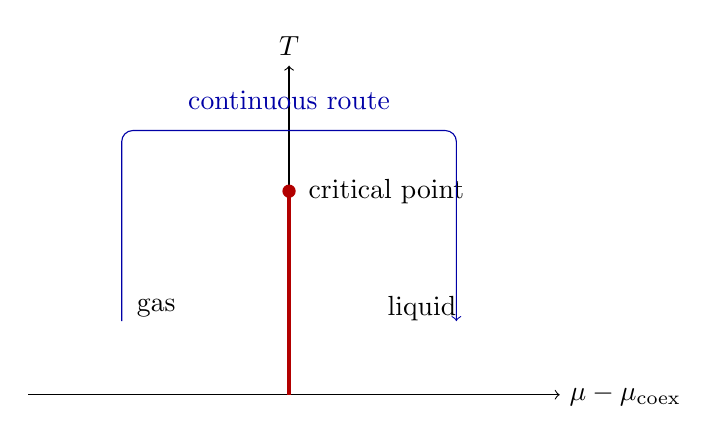
\begin{tikzpicture}[x=1.25cm,y=1.1cm]
\draw[->] (-2.65,0) -- (2.75,0) node[right] {$\mu-\mu_{\rm coex}$};
\draw[->] (0,0) -- (0,3.8) node[above] {$T$};
\draw[very thick,red!70!black] (0,0) -- (0,2.35);
\fill[red!70!black] (0,2.35) circle (2.4pt);
\node[right] at (0.1,2.35) {critical point};
\node at (-1.35,1.0) {gas};
\node at (1.35,1.0) {liquid};
\draw[->,blue!65!black,rounded corners]
 (-1.7,0.85) -- (-1.7,3.05) -- (1.7,3.05) -- (1.7,0.85);
\node[blue!65!black] at (0,3.4) {continuous route};
\end{tikzpicture}
\caption{Flüssigkeit und Gas sind unterhalb des Endpunkts verschiedene Phasen, doch im überkritischen Bereich trennt sie keine singuläre Phasengrenze.}
\label{fig:liquid-gas-plane}
\end{figure}

Damit ist die vertraute Siedelinie identifiziert. Erhitzt man eine Flüssigkeit bei festem Druck, bis sie die Koexistenzlinie überschreitet, beginnt sie zu sieden. Auch bei fester Temperatur kann man durch eine Änderung des Drucks oder des chemischen Potenzials dieselbe Grenze überschreiten. Ein überhitzter Dampf oder eine unterkühlte Flüssigkeit ist eine metastabile Fortsetzung jenseits der Gleichgewichtskoexistenz; für die Beschreibung ihrer Lebensdauer braucht man die Nukleationsdynamik, die über diese Gleichgewichtskonstruktion hinausgeht.

\begin{classroomqa}
\audiencequestion{Ist überhitzter Dampf in diesem Phasendiagramm dargestellt?}
\lecturerresponse{Das Gleichgewichtsdiagramm zeigt die Koexistenzgrenze. Ein überhitzter oder übersättigter Zustand ist metastabil: Er bleibt vorübergehend auf der falschen Seite bestehen, weil die Bildung eines kritischen Tröpfchens eine Grenzflächen-Freienergie kostet. Diese kinetische Verfeinerung wird hier nicht berechnet. \lecturetimestamp{01:12:19--01:12:29}}
\end{classroomqa}

\begin{classroomqa}
\audiencequestion{Wie lässt sich das chemische Potenzial in einem gewöhnlichen Fluid verändern?}
\lecturerresponse{Der Behälter mit der Potenzialmulde ist eine klare theoretische Kontrollmöglichkeit. Im Labor verändert man häufiger den Druck oder das Volumen oder stellt Kontakt mit einem Reservoir her; die Thermodynamik übersetzt diese Änderungen dann in eine Änderung des chemischen Potenzials. \lecturetimestamp{01:12:30--01:13:59}}
\end{classroomqa}

\begin{classroomqa}
\audiencequestion{Ändert sich mit der Dichte auch das molekulare Potenzial \(J\)?}
\lecturerresponse{Nein. Bei einem festen Stoff beschreibt \(J\) die kurzreichweitige Anziehung und bleibt in diesem Modell unverändert. Eine Änderung von \(\mu\) verändert die Zahl der besetzten Gitterplätze und damit die Verteilung der intermolekularen Abstände. Eine Änderung von \(J\) würde bedeuten, den mikroskopischen Stoff oder die Wechselwirkung zu ändern. \lecturetimestamp{01:14:50--01:15:41}}
\end{classroomqa}

\begin{classroomqa}
\audiencequestion{Ist die kritische Temperatur dasselbe wie der gewöhnliche Siedepunkt?}
\lecturerresponse{Nein. Ein Siedepunkt ist für einen bestimmten Druck festgelegt und verschiebt sich daher mit dem Druck entlang der Koexistenzkurve. Die kritische Temperatur ist der eindeutige Endpunkt, oberhalb dessen Flüssigkeit und Gas nicht mehr durch eine Phasengrenze getrennt sind. Der Druck wurde in dieser Behandlung des Gittergases nicht explizit hergeleitet. \lecturetimestamp{01:15:42--01:17:02}}
\end{classroomqa}

Nun lässt sich das zentrale Ergebnis formulieren. Ising-Magnet und Gittergas zeichnen nicht bloß ähnliche Diagramme. Nach einer Änderung der Variablen und Parameter besitzen sie dieselbe Zustandssumme. Jeder singulären thermodynamischen Eigenschaft auf der einen Seite entspricht eine auf der anderen:
\begin{equation}
\begin{array}{c|c}
\text{Ising magnet} & \text{lattice gas}\\ \hline
\sigma_i=\pm1 & n_i=0,1\\
m=\expect{\sigma} & \rho=(1+m)/2\\
h & \mu=-(4dJ+2h)\\
\text{aligned exchange} & \text{nearest-neighbor attraction}\\
h=0,\ T<T_c & \text{liquid--gas coexistence}\\
(T_c,0) & \text{critical endpoint}
\end{array}
\label{eq:ising-fluid-dictionary}
\end{equation}

\section{Kritische Exponenten und Universalität}

Nahe einem kritischen Punkt zeigen thermodynamische Größen oft Potenzgesetz-Singularitäten. Mit der reduzierten Temperatur
\begin{equation}
t=\frac{T-T_c}{T_c},
\end{equation}
schreibt man schematisch
\begin{equation}
m\sim(-t)^{\beta_{\rm crit}},
\qquad
\chi\sim |t|^{-\gamma},
\qquad
\xi\sim |t|^{-\nu}.
\label{eq:critical-exponents}
\end{equation}
Dabei ist \(\beta_{\rm crit}\) ein kritischer Exponent und keine inverse Temperatur. Die Mean-Field-Näherung ergibt \(\beta_{\rm crit}=1/2\), doch Fluktuationen verändern die Exponenten unterhalb der oberen kritischen Dimension.

Die Exponenten müssen keine ganzen Zahlen sein. Sie müssen allerdings auch nicht alle irrational sein: Das zweidimensionale Ising-Modell hat bekanntermaßen mehrere exakte rationale Exponenten, während die Werte für das dreidimensionale Ising-Modell nichttriviale Zahlen sind, die sich mithilfe von Theorie und numerischen Rechnungen mit hoher Präzision bestimmen lassen. Die robuste Erkenntnis ist, dass die Exponenten im Allgemeinen nicht durch elementare Dimensionsanalyse festgelegt sind.

Noch bemerkenswerter ist, dass sie oft auch nicht von den mikroskopischen Details abhängen. Systeme mit derselben räumlichen Dimension und derselben Symmetrie des Ordnungsparameters sowie hinreichend kurzreichweitigen Wechselwirkungen können zu derselben kritischen Theorie auf großen Längenskalen fließen. Sie gehören derselben \emph{Universalitätsklasse} an. Sowohl ein uniaxialer Magnet als auch der kritische Endpunkt eines gewöhnlichen Flüssigkeit--Gas-Systems haben einen skalaren Ordnungsparameter und gehören in derselben Dimension zur Ising-Universalitätsklasse.

\begin{classroomqa}
\audiencequestion{Gibt es eine endliche oder diskrete Liste von Universalitätsklassen?}
\lecturerresponse{Es gibt viele Klassen, geordnet nach Dimension, Symmetrien, Erhaltungssätzen, Reichweite der Wechselwirkungen und weiteren Eigenschaften auf großen Längenskalen. In vielen vertrauten Fällen sind die Fixpunkte und Exponentensätze diskret, doch es gibt auch Systeme mit stetig variierenden Exponenten. Die sichere Aussage lautet nicht, dass die Liste endlich ist, sondern dass viele mikroskopisch unterschiedliche Systeme dieselben Eigenschaften auf großen Längenskalen aufweisen. \lecturetimestamp{01:18:50--01:19:38}}
\end{classroomqa}

\begin{classroomqa}
\audiencequestion{Wenn Flüssigkeit und Gas koexistieren, was trennt sie in einem tatsächlichen Behälter?}
\lecturerresponse{Eine Grenzfläche. Die Oberflächenspannung macht Grenzflächenfläche energetisch ungünstig, während die Schwerkraft einen vertikalen Gradienten des chemischen Potenzials erzeugt und die dichtere Flüssigkeit gewöhnlich unterhalb des Gases anordnet. Bei vernachlässigbarer Schwerkraft wird die Geometrie unmittelbarer durch die Oberflächenspannung und die Randbedingungen bestimmt. \lecturetimestamp{01:19:40--01:21:18}}
\end{classroomqa}

\begin{classroomqa}
\audiencequestion{Wo kommt in diesem Bild die Verdampfungswärme vor?}
\lecturerresponse{Unterhalb des kritischen Punkts ist das Überschreiten der Erstordnungs-Koexistenzlinie im Allgemeinen mit latenter Wärme verbunden. Die Verdampfungswärme geht gegen null, wenn man sich dem kritischen Endpunkt nähert, denn dort werden die beiden Phasen identisch. In dieser Vorlesung wird die Phasenstruktur hergeleitet, die latente Wärme jedoch nicht berechnet. \lecturetimestamp{01:21:19--01:22:18}}
\end{classroomqa}

\begin{classroomqa}
\audiencequestion{Kann man einen Phasenübergang als empfindlichen Detektor nutzen, zum Beispiel mit einer supraleitenden Vorrichtung?}
\lecturerresponse{Ja. In der Nähe eines Übergangs kann eine kleine Störung eine starke Reaktion hervorrufen oder einen Zustandswechsel auslösen. Praktische Detektoren nutzen diese Empfindlichkeit, auch wenn der relevante Ordnungsparameter und die Dynamik sich vom Ising-Beispiel unterscheiden können. \lecturetimestamp{01:22:19--01:24:05}}
\end{classroomqa}

Damit ist der Kurs über statistische Mechanik abgeschlossen. Er begann mit Entropie und Gleichgewicht, führte über Zustandssummen und Gase und zeigte schließlich, dass ein Magnet und ein Fluid zwei Beschreibungen desselben kritischen Phänomens sein können.

\section{Nachgespräch zur Vorlesung: Feinabstimmung und Selektion}

Nach dem Ende der eigentlichen Vorlesung wurde das Gespräch noch ungefähr vierzig Minuten fortgesetzt. Es lohnt sich, es festzuhalten, doch sollte man es nicht mit der obigen Herleitung verwechseln. Es geht nun nicht mehr um das Gittergas, sondern um die Logik der Feinabstimmung und den vorsichtigen Einsatz anthropischer Selektion in der Kosmologie.

\subsection{Kleine Zahlen sind nicht automatisch feinabgestimmt}

Es gibt keinen einzelnen Satz, der jeden Gebrauch des Ausdrucks \emph{anthropisches Prinzip} abschließend klärt. Ein sinnvoller Ausgangspunkt ist eine operationale Formulierung: Wenn eine Theorie viele tatsächlich verwirklichte Umgebungen zulässt, sind Beobachtungen durch die Tatsache bedingt, dass Beobachter nur in einigen davon entstehen können. Diese bedingte Aussage kann vernünftig sein. Sie bleibt inhaltsleer, wenn man sie ohne ein Ensemble, eine Selektionsbedingung oder einen Mechanismus anführt, der den Alternativen physikalische Bedeutung verleiht.

Bevor Selektion ins Spiel kommt, muss man zwischen einem kleinen Parameter und einem feinabgestimmten Parameter unterscheiden. Ein Wert kann klein sein, weil ein stabiler dynamischer Mechanismus ihn auf einen besonderen Wert einstellt. Feinabstimmung bedeutet, dass der beobachtete Wert eine außerordentlich genaue Balance zwischen ansonsten unabhängigen Beiträgen zu erfordern scheint, ohne dass ein bekannter rückstellender Mechanismus oder eine Symmetrie diese Balance schützt.

\begin{classroomqa}
\audiencequestion{Lässt sich das anthropische Prinzip präzise formulieren?}
\lecturerresponse{Sein vertretbarer Gebrauch ist bedingt, nicht mystisch: Wenn viele physikalisch verwirklichte Umgebungen unterschiedliche Parameter haben, stammen die von Wesen wie uns beobachteten Umgebungen aus der Teilmenge, die mit der Existenz von Beobachtern vereinbar ist. Das erzeugt weder die Umgebungen noch weist es ihnen Wahrscheinlichkeiten zu; dafür ist die zugrunde liegende Physik zuständig. \lecturetimestamp{01:25:45--01:26:13}}
\end{classroomqa}

Die kosmologische Konstante ist das maßgebliche Beispiel. Ihr beobachteter Betrag ist im Vergleich zu den naiven Beiträgen der Quantenfeldtheorie zur Vakuumenergie außerordentlich klein. Das Problem besteht nicht allein darin, dass der Endwert klein ist. Vielmehr scheinen sich viele große Terme mit enormer Genauigkeit aufzuheben, während kein anerkanntes Rückkopplungsverfahren bei niedrigen Energien das Ergebnis auf den beobachteten Wert einstellt.

\subsection{Das Luftschiff und das U-Boot}

Zwei Beispiele zum Auftrieb machen den Unterschied deutlich. Ein Luftschiff schwebt in einer Höhe, in der seine mittlere Dichte der Dichte der umgebenden Luft entspricht. Mit zunehmender Höhe nimmt die Luftdichte ab. Steigt das Luftschiff, wird die Außenluft weniger dicht und das Luftschiff sinkt tendenziell wieder; sinkt es, wird die Außenluft dichter und das Luftschiff steigt tendenziell wieder. Der Dichteausgleich mag numerisch empfindlich sein, doch der Dichtegradient der Atmosphäre sorgt für eine rückstellende Rückkopplung. Das Gleichgewicht ist dynamisch erklärt.

Ein in nahezu inkompressiblem Wasser schwebendes U-Boot verhält sich anders. Die Wasserdichte ändert sich mit der Tiefe nur wenig. Falls die mittlere Dichte des U-Boots zufällig der des umgebenden Wassers entspricht, gibt es keinen vergleichbaren tiefenabhängigen Rückstellmechanismus, der diese Gleichheit erklärt. Schon eine winzige Abweichung lässt es steigen oder sinken. Um den Schwebezustand zu erreichen, müssen Ballast und Inhalt präzise angepasst werden. Der kleine Restunterschied ist dann feinabgestimmt, sofern ihn kein Regelsystem oder Konstruktionsmechanismus erklärt.

\begin{figure}[ht]\centering
\resizebox{\linewidth}{!}{%
\begin{tikzpicture}[>=Latex]
\begin{scope}[xshift=-3.8cm]
\shade[top color=blue!5,bottom color=blue!28] (-2.5,-2.2) rectangle (2.5,2.2);
\draw[very thick,rounded corners=18pt,fill=yellow!35]
  (-1.15,0) ellipse (1.15 and 0.55);
\draw[thick] (0,-0.55) -- (0,-1.05);
\draw[thick,fill=gray!20] (-0.45,-1.05) rectangle (0.45,-1.38);
\draw[->,red!70!black,thick] (1.65,1.45) -- (1.65,0.55)
 node[midway,right] {restoring};
\draw[->,red!70!black,thick] (-1.65,-1.45) -- (-1.65,-0.55)
 node[midway,left] {restoring};
\node at (0,2.55) {\textbf{Blimp: density gradient}};
\node[align=center] at (0,-2.75) {displacement changes\\the buoyant imbalance};
\end{scope}
\begin{scope}[xshift=3.8cm]
\shade[top color=cyan!10,bottom color=blue!45] (-2.5,-2.2) rectangle (2.5,2.2);
\draw[very thick,fill=gray!35,rounded corners=12pt]
  (-1.45,-0.25) -- (1.1,-0.25) arc (-90:90:0.38)
  -- (-1.45,0.51) -- cycle;
\draw[thick] (-0.25,0.51) -- (-0.25,0.85) -- (0.35,0.85) -- (0.35,0.51);
\draw[->,red!70!black,thick] (1.65,0.15) -- (1.65,1.35)
 node[midway,right] {rise};
\draw[->,red!70!black,thick] (-1.65,0.15) -- (-1.65,-1.35)
 node[midway,left] {sink};
\node at (0,2.55) {\textbf{Submarine: nearly uniform density}};
\node[align=center] at (0,-2.75) {no depth-dependent feedback\\protects neutral buoyancy};
\end{scope}
\end{tikzpicture}}\caption{Ein kleiner Dichteunterschied kann dynamisch stabil oder tatsächlich feinabgestimmt sein. Beim Luftschiff wirkt eine rückstellende Rückkopplung; beim idealisierten U-Boot muss die mittlere Dichte an die des Wassers angepasst werden.}\label{fig:blimp-submarine}\end{figure}

\begin{classroomqa}
\audiencequestion{Warum sollte die Besatzung des U-Boots eine Erklärung verlangen, wenn neutrale Auftriebskraft beobachtet wird?}
\lecturerresponse{Denn ohne einen Ballastregelmechanismus schützt weder eine Symmetrie noch eine Rückkopplung aus der Umgebung die Gleichheit zweier unabhängiger Dichten. Die Frage ist nicht, ob diese Gleichheit logisch möglich ist, sondern warum sich das System in einem so engen Bereich seines Parameterraums befindet. \lecturetimestamp{01:35:05--01:36:25}}
\end{classroomqa}

\subsection{Viele Bereiche und bedingte Beobachtung}

Stellen wir uns nun einen Prozess vor, der eine enorme Zahl von U-Booten mit vielen verschiedenen mittleren Dichten hervorbringt. Die meisten sinken oder steigen; nur ein winziger Bruchteil bleibt längere Zeit im bewohnbaren Bereich zwischen Oberfläche und Meeresboden. Ein Beobachter, der notwendigerweise in einem der überlebenden U-Boote lebt, sollte sich nicht wundern, nahezu neutralen Auftrieb zu messen. Die Beobachtung ist durch die Bedingung selektiert, die für die Anwesenheit des Beobachters erfüllt sein muss.

Diese Überlegung erfordert zwei Bestandteile:
\begin{enumerate}
\item einen physikalischen Prozess, der tatsächlich viele Alternativen verwirklicht, statt sie nur in der Vorstellung bestehen zu lassen;
\item eine Selektionsbedingung, die erklärt, warum Beobachtungen nur in einer eingeschränkten Teilmenge gemacht werden.
\end{enumerate}
Selektion ersetzt den Erzeugungsmechanismus nicht. Sie verändert die bedingte Wahrscheinlichkeit dafür, was ein Beobachter misst, sobald das Ensemble existiert.

\begin{classroomqa}
\audiencequestion{Läuft das Argument nicht bloß darauf hinaus, dass Unwahrscheinliches irgendwo in einer ausreichend großen Stichprobe vorkommt?}
\lecturerresponse{Das ist nur die erste Hälfte. Die zweite ist die bedingte Betrachtung von Beobachtungen: Beobachter werden nicht gleichmäßig aus allen Bereichen ausgewählt, sondern nur aus solchen, in denen ihre Existenz möglich ist. Ein vollständiger Vorschlag benötigt weiterhin ein Maß über die Bereiche und eine physikalische Erklärung dafür, wie sie entstehen. \lecturetimestamp{01:39:19--01:40:36}}
\end{classroomqa}

Auf die Vakuumenergie angewandt bedeutet dies: Eine große negative kosmologische Konstante kann dazu führen, dass ein Universum zu rasch wieder kollabiert, während ein hinreichend großer positiver Wert die Materie daran hindern kann, sich zu Galaxien zu verdichten. Der beobachtete Wert liegt in dem engen Bereich, der mit langlebigen Strukturen vereinbar ist. Das liefert eine mögliche Selektionsbedingung, aber keine Herleitung der Verteilung kosmologischer Konstanten.

Die Quantenfeldtheorie bringt das Feinabstimmungsproblem hinzu: Die Vakuumbeiträge verschiedener Felder und Energieskalen sind einzeln viel größer als der beobachtete Restwert. Wenn sich diese Terme nahezu exakt aufheben, ähnelt das Ergebnis eher dem sorgfältig austarierten U-Boot als dem selbstregulierenden Luftschiff. Die Analogie soll das logische Problem sichtbar machen, nicht dessen Lösung liefern.

\begin{classroomqa}
\audiencequestion{Können Änderungen eines Parameters durch Änderungen mehrerer anderer ausgeglichen werden?}
\lecturerresponse{Ja. Die Menge zulässiger Parameterwerte muss kein enges Intervall auf einer einzelnen Achse sein; sie kann eine dünne Fläche in einem mehrdimensionalen Parameterraum bilden. Korrelierte Änderungen können Strukturen erhalten. Dann stellt sich jedoch die Frage, warum die verwirklichten Parameter nahe dieser Fläche liegen und welches Maß ihnen die zugrunde liegende Theorie zuweist. \lecturetimestamp{01:45:10--01:46:19}}
\end{classroomqa}

\begin{figure}[ht]\centering
\begin{tikzpicture}[x=1.3cm,y=1.05cm,>=Latex]
\draw[->] (-3.2,0) -- (3.4,0) node[right] {$\lambda_1$};
\draw[->] (0,-2.5) -- (0,2.65) node[above] {$\lambda_2$};
\fill[gray!12] (-3,-2.25) rectangle (3.1,2.3);
\draw[very thick,blue!65!black]
 (-2.8,-1.55) .. controls (-1.3,-0.75) and (0.15,0.05) .. (2.85,1.55);
\draw[very thick,blue!25]
 (-2.8,-1.25) .. controls (-1.3,-0.45) and (0.15,0.35) .. (2.85,1.85);
\fill[blue!15,opacity=.65]
 (-2.8,-1.55) .. controls (-1.3,-0.75) and (0.15,0.05) .. (2.85,1.55)
 -- (2.85,1.85) .. controls (0.15,0.35) and (-1.3,-0.45) .. (-2.8,-1.25) -- cycle;
\node[blue!65!black,rotate=28] at (1.3,0.95) {viable band};
\foreach \x/\y in {-2.4/1.45,-1.7/-1.8,-0.9/1.8,0.3/-1.45,1.2/1.85,2.4/-0.8}
  \fill[red!65!black] (\x,\y) circle (2pt);
\fill[green!45!black] (0.55,0.58) circle (2.8pt);
\node[green!35!black,right] at (0.65,0.55) {observed domain};
\end{tikzpicture}\caption{Bei mehreren Parametern kann die Bewohnbarkeit oder strukturelle Stabilität in einem schmalen korrelierten Band liegen, statt in einem engen Intervall eines einzelnen Parameters. Selektion beschränkt die Beobachtungen auf dieses Band, erzeugt aber nicht die Parameterverteilung.}\label{fig:viable-parameter-band}\end{figure}

\subsection{Landschaftsmodelle und ihre Unsicherheiten}

Als mögliche Quelle von Alternativen wird eine Theorie mit vielen metastabilen Vakuumzuständen vorgeschlagen, die möglicherweise in verschiedenen kosmologischen Bereichen besetzt werden. Ideen einer Landschaft in der Stringtheorie und Szenarien ewiger Inflation sind Beispiele dafür; ihre konkrete Verwirklichung und das zugehörige Wahrscheinlichkeitsmaß sind jedoch weiterhin unsicher. In der Vorlesung wird dies als Möglichkeit dargestellt, nicht als gesicherte Tatsache.

Eine Symmetrie wäre eine konventionellere Erklärung, wenn sie die kosmologische Konstante zwingend auf null setzte. Die Schwierigkeit besteht darin, dass die beobachtete beschleunigte Expansion einem kleinen, aber von null verschiedenen Wert entspricht. Ein Mechanismus, der auf natürliche Weise exakt null ergibt, erklärt nicht automatisch einen winzigen Restwert; durch Symmetriebrechung kann die Feinabstimmung einfach wiederkehren. Hier kommt das Bild des U-Boots zurück: Ein Seil könnte es in einer bestimmten Tiefe halten, doch dann muss man den Mechanismus, den das Seil darstellt, identifizieren, statt ihn einfach vorauszusetzen.

\begin{classroomqa}
\audiencequestion{Verstößt eine sehr genaue Messung eines Parameters gegen die Unschärferelation?}
\lecturerresponse{Nein. Eine Unschärferelation gilt für bestimmte Paare nicht kommutierender Observablen. Eine Kopplungskonstante oder ein Vakuumparameter kann einen scharf definierten Wert haben, ohne zu einer unkontrollierten Observablen kanonisch konjugiert zu sein. Hohe Messgenauigkeit ist für sich genommen kein Paradox der Unschärferelation. \lecturetimestamp{01:49:21--01:49:36}}
\end{classroomqa}

\begin{classroomqa}
\audiencequestion{Erklärt anthropisches Schließen den Wert oder wiederholt es nur, dass Beobachter ihn voraussetzen?}
\lecturerresponse{Selektion allein ist keine dynamische Erklärung. Ihre legitime Rolle besteht darin, bedingte Wahrscheinlichkeiten in einem physikalisch verwirklichten Ensemble zu verändern. Ohne Ensemble, Maß oder überprüfbare Konsequenzen droht sie zu einer bloßen Bezeichnung statt zu einer Erklärung zu werden. \lecturetimestamp{01:49:37--01:50:21}}
\end{classroomqa}

\subsection{Mäßige Koinzidenzen in der Teilchenphysik}

Gewöhnliche Materie, wie wir sie kennen, hängt von Photonen, Elektronen, leichten Quarks und der starken Wechselwirkung ab; Neutrinos beeinflussen die Kosmologie, sind aber keine direkten Bindungspartner der Atome. Besonders folgenreich ist die Proton--Neutron-Massendifferenz. Da das Neutron etwas schwerer als das Proton ist, können freie Neutronen zerfallen, während gewöhnlicher Wasserstoff stabil ist. Eine hinreichend starke Umkehrung dieser Reihenfolge würde die Kernchemie grundlegend verändern.

Auch die Elektronenmasse und die Feinstrukturkonstante bestimmen Atomgrößen und Bindungsenergien. Eine erhebliche Änderung würde die Chemie verändern. Das sind bedeutsame Aussagen über Empfindlichkeit, doch sollte man sie nicht zu der Behauptung überhöhen, jede kleine Änderung schließe jede denkbare Form von Komplexität aus. Im Vergleich zum Problem der kosmologischen Konstante sind viele dieser Koinzidenzen mäßig und mit anderen Parametern korreliert.

Das mit der elektroschwachen Skala verbundene Hierarchieproblem ist ein weiteres prominentes Natürlichkeitsproblem: Strahlungskorrekturen machen die Masse eines fundamentalen Skalarfelds tendenziell empfindlich gegenüber hohen Energieskalen, sofern sie nicht durch zusätzliche Strukturen geschützt ist. Sein Status und seine Deutung unterscheiden sich vom Problem der Vakuumenergie; keines von beiden sollte auf ein Schlagwort reduziert werden.

\begin{classroomqa}
\audiencequestion{Wäre eine Änderung der Proton--Neutron-Massendifferenz für gewöhnliche Materie wirklich von Bedeutung?}
\lecturerresponse{Ja. Die beobachtete Reihenfolge ermöglicht stabilen Wasserstoff und bestimmt die Betastabilität der verschiedenen Atomkerne. Schon mäßige Änderungen können die Kernhäufigkeiten und die Energieerzeugung in Sternen neu ordnen. Bei einer sorgfältigen Analyse müssen die gekoppelten Parameter konsistent variiert werden, statt einen einzelnen Wert zu ändern und alle anderen festzuhalten. \lecturetimestamp{01:51:47--01:53:08}}
\end{classroomqa}

\begin{classroomqa}
\audiencequestion{Welche Rolle spielen die Elektronenmasse und die Feinstrukturkonstante?}
\lecturerresponse{Sie legen charakteristische atomare Energie- und Längenskalen fest, schematisch \(E_{\rm atom}\sim \alpha^2m_e\) und \(a_0\sim(\alpha m_e)^{-1}\) in den Einheiten \(\hbar=c=1\). Große Änderungen würden die Chemie grundlegend verändern, auch wenn der genaue zulässige Bereich eine mehrdimensionale Frage ist. \lecturetimestamp{01:53:09--01:54:12}}
\end{classroomqa}

\subsection{Kontroversen, Zeitabhängigkeit und Überprüfbarkeit}

Das Gespräch wendet sich kurz der Kritik an der Inflationstheorie und der Deutung präziser kosmologischer Daten zu. Diese historische Kontroverse sollte als Kontroverse dargestellt und nicht durch Rhetorik entschieden werden. Die Inflationstheorie hat erfolgreiche phänomenologische Vorhersagen und viele Modellvarianten; Fragen zu Anfangsbedingungen, Wahrscheinlichkeitsmaßen und Überprüfbarkeit bleiben offen. Daten schränken die Modelle ein, aber ein einzelner beiläufiger Verweis auf ein Experiment entscheidet nicht über den gesamten theoretischen Rahmen.

\begin{classroomqa}
\audiencequestion{Könnte sich die kosmologische Konstante langsam mit der Zeit ändern, statt konstant zu sein?}
\lecturerresponse{Ein dynamisches Dunkle-Energie-Feld kann eine zeitabhängige beschleunigte Expansion hervorrufen. Es bringt ein Potenzial und Anfangsbedingungen mit sich, die ihrerseits erklärt werden müssen, und Beobachtungen schränken die Zustandsgleichung auf Werte nahe denen einer kosmologischen Konstante ein. Zum Zeitpunkt der Vorlesung gab es keinen Hinweis, der eine nennenswerte zeitliche Änderung erforderte. \lecturetimestamp{01:57:17--01:59:19}}
\end{classroomqa}

\begin{classroomqa}
\audiencequestion{Löst anthropische Selektion selbst die Nukleation verschiedener Universen oder Bereiche aus?}
\lecturerresponse{Nein. Selektion besagt, welche verwirklichten Bereiche Beobachter enthalten können; sie erzeugt diese Bereiche nicht. Ein eigenständiger kosmologischer Mechanismus, etwa Vakuumübergänge im Verlauf einer inflationären Entwicklung, müsste sie hervorbringen. \lecturetimestamp{01:59:20--01:59:42}}
\end{classroomqa}

Die kausale Reihenfolge muss klar bleiben:
\begin{equation}
\begin{gathered}
\text{laws and initial conditions}\\[-0.15em]
\downarrow\\[-0.15em]
\text{physical environments}\\[-0.15em]
\downarrow\\[-0.15em]
\text{observers and observations}
\end{gathered}
\end{equation}
Beobachter reichen nicht rückwärts in der Zeit und bestimmen die Naturgesetze. Die Konditionierung kommt ins Spiel, wenn wir fragen, was ein aus den verwirklichten Umgebungen ausgewählter Beobachter wahrscheinlich messen wird.

Die wissenschaftliche Frage lautet daher nicht, ob die Ausdrucksweise philosophisch, politisch oder religiös klingt. Entscheidend ist, ob der Vorschlag ein klar definiertes physikalisches Ensemble, ein berechenbares oder zumindest eingeschränktes Maß und Konsequenzen aufweist, die ihn von Alternativen unterscheiden könnten. Als mögliche Signaturen einer Kosmologie mit mehreren Vakuumzuständen werden Spuren von Kollisionen zwischen Blasenbereichen diskutiert. Solche Signale lassen sich nur schwer zuverlässig vorhersagen; im Rahmen der Diskussion zur Zeit der Vorlesung war kein derartiger Nachweis im kosmischen Mikrowellenhintergrund erbracht worden. Das Fehlen eines einfachen Tests ist eine ernsthafte Einschränkung, aber kein Grund, die Idee für wahr zu erklären oder das zugrunde liegende Feinabstimmungsproblem abzutun.

\begin{classroomqa}
\audiencequestion{Was müsste aus diesem Selektionsargument eine wissenschaftliche Theorie machen?}
\lecturerresponse{Der Vorschlag benötigt einen Mechanismus, der die Alternativen erzeugt, ein Wahrscheinlichkeitsmaß oder einen kontrollierten Ersatz dafür sowie beobachtbare Konsequenzen. Signaturen von Blasenkollisionen sind eine mögliche Forschungsrichtung; ihr Ausbleiben oder ihre Mehrdeutigkeit zeigt jedoch, wie anspruchsvoll das Problem der Überprüfbarkeit ist. \lecturetimestamp{02:02:31--02:04:12}}
\end{classroomqa}

Das Nachgespräch endet mit dieser nüchternen Feststellung. Feinabstimmung ist ein Hinweis darauf, dass möglicherweise eine Erklärung fehlt. Symmetrie, dynamische Anpassung und Selektion durch die Umgebung sind logisch verschiedene mögliche Erklärungen. Selektion kann vernünftig sein, aber nur als Bestandteil einer physikalischen Erklärung, deren Annahmen und Grenzen offen dargelegt werden.
